% Paridyum mark, as vector geometry.
%
% Built rather than embedded so it stays sharp at the 1.9cm the letterhead
% sets it at, and so it carries no raster artefacts into a legal document.
% Rebuild with:  pdflatex -output-directory=latex/assets latex/assets/paridyum-logo.tex
%
% Two quarter discs sharing a corner: the large one opening up and right,
% the small one opening down and left, separated by a thin notch.
\documentclass[border=0pt]{standalone}
\usepackage{tikz}

\begin{document}
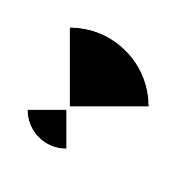
\begin{tikzpicture}[x=1cm, y=1cm]
  \definecolor{paridyumink}{HTML}{000000}

  \pgfmathsetmacro{\R}{1.00}   % large quarter disc radius
  \pgfmathsetmacro{\s}{0.49}   % small quarter disc radius
  \pgfmathsetmacro{\g}{0.045}  % notch between the two

  % Large: right angle at the origin, arc sweeping from top to right.
  \fill[paridyumink]
    (0,0) -- (0,\R) arc[start angle=90, end angle=0, radius=\R] -- cycle;

  % Small: right angle at the origin offset by the notch, opening down-left.
  \begin{scope}[shift={(-\g,-\g)}]
    \fill[paridyumink]
      (0,0) -- (-\s,0) arc[start angle=180, end angle=270, radius=\s] -- cycle;
  \end{scope}
\end{tikzpicture}
\end{document}
